\documentclass[]{article}
\usepackage[utf8]{inputenc}
\usepackage[slovak]{babel}
\usepackage[hidelinks]{hyperref}
\usepackage{graphicx}

\begin{document}
	
	\begin{titlepage}
		\begin{center}
			\textsc{{\LARGE Vysoké učení technické v~Brně\\[0.3em]
					Fakulta informačních technologií}}\\
			\vspace{\stretch{0.382}}
			{\Huge \textbf{ITU -- Technická správa}\\[0.2em]Time Tracker}
			\vspace{\stretch{0.618}}
		\end{center}
		
		\noindent Číslo projektu: 103\\
		Číslo a názov tímu: 11, Tým xbolva00\\
		Autor: Dávid Bolvanský (xbolva00)\\
		Ďalší členova tímu: Martin Marušiak (xmarus07), Juraj Ondrej Dúbrava (xdubra03)\\
\end{titlepage}

\tableofcontents

\newpage

\section{Abstrakt}
Cieľom projektu je vytvoriť program Time Tracker, čo je program slúžiaci na sledovanie činností užívateľa na počítači. Dôraz je kladený na vytvorenie jednoduchého programu s~nenáročným ovládaním, ktorý ponúkne základné ale aj pokročilé vlastnosti. 

Program je určený ľudom, ktorí chcú mať prehľad o~činnostiach vykonaných či prebiehajúcich na počítači, a to za účelom lepšej organizácie činností a ich efektívnejšej realizácie. Užívateľovi bude k~dispozícii prehľad o~činnostiach, bude možné zobraziť podrobné informácie o~danej činnosti. Taktiež bude k~dispozícii možnosť zobrazenia prehľadu za určité časové obdobie. Užívateľ bude taktiež si vytvoriť vlastný plán činností, a následne program môže upozorniť používateľa na nezhody medzi plánom a skutočnosťou. Rovnako je aplikácia určená pre ľudí, ktorí chcú vedieť aké činnosti sa na ich počítači vykonávali a poprípade tieto vykonávané činnosti mohli spoplatniť.

Najväčšími pozitívami programu by mali byť vlastnosti ako sú multiplatformovosť aplikácie, automatické sledovanie procesov a programov, tvorba vlastného TODO listu a kategorizácia činností, upozornenia na nezhody s~plánom, t.j. prekročená očakávaná doba trvania danej aktivity a možnosť zobrazenia prehľadných štatistík o~aktivitách a kategóriách.

\newpage

\section{Prieskum kontextu použitia}

Skúmame, kto je naša cieľová skupina, aké vlastnosti má typický používateľ a čo očakáva od programu, prípady použitia programu. Zisťujeme informácie o~cieľovom prostredí, analyzujeme existujúce riešenia a skúmame ich výhody a nevýhody.

\subsection{Cieľová skupina}
Produkt bude zameraný hlavne na jednotlivcov, ktorí chcú mať pod kontrolou čas strávený pri jednotlivých činnostiach za počítanom a na základe tejto informácie optimalizovať svoj harmonogram činností. Užívatelia si svoje aktivity na počítači plánujú, kategorizujú a radi skúmajú to akým spôsobom čas strávili. Nedarí sa im však dodržiavať plány, a preto potrebujú nástroj, ktorý by im v~tom pomohol. Produkt môžu využiť aj ľudia, ktorý si účtujú prácu na počítači od časovej jednotky, napr. pre freelancerov\footnote{\url{https://en.wikipedia.org/wiki/Freelancer}}, aby vedeli, koľko si za prácu môžu zaúčtovať. Alebo naopak pre sledovanie výdavkov pri používaní plateného softvéru.	 


\subsection{Typický užívateľ}
Typický používateľ je v~produktívnom veku (18--60), počítač používa každý deň za účelom práce alebo štúdia. Čas strávený za počítačom tvorí značnú časť celého dňa, a preto tento užívateľ chce mať prehľad o~svojich činnostiach v~rámci určitého časového obdobia, aby pomer práce k~času (vykonaná práca za daný čas) bol vyšší, t.j. za rovnaký čas urobiť viac a lepšie (efektívnejšia, kvalitnejšia práca), a pod.

\newpage

\subsubsection{Persóna typického užívateľa}
Peter má 21 rokov a je študentom VŠ v~odbore informatika. Je freelancerom, popri štúdiu si privyrába si tvorbou webových stránok. Peter venuje hlavnú časť svojho úsilia škole a tvorbe stránok, preto trávi na počítači množstvo času. Svoje aktivity si vždy plánuje aby mohol efektívne rozdeliť čas, ktorý venuje jednotlivým činnostiam. Vie, že niekedy strávi príliš dlho času nad jednou činnosťou a nezostane mu čas na ostatné veci. Inokedy si zase Peter naplánuje príliš mnoho vecí a splní len pár, pretože nedokáže predom dobre odhadnúť koľko mu zaberú. Peter preferuje poriadok a pevný rád, vytvára si záložky a kategorizuje. Preto potrebuje nástroj, ktorý by kontroloval ako prebieha plnenie úloh a prípadne ho upozornil na odchýlku v~pláne, nástroj by mu taktiež mal poskytnúť spätnú väzbu aby mohol svoje činnosti lepšie plánovať a kategorizovať.

Peter si počas tvorby stránok často zapisuje aj čas strávený ich tvorbou, čo berie do úvahy pri vyúčtovaní s~klientom. Chcel by teda nástroj, ktorý by na základe stráveného času automaticky odvodil finančnú čiastku, ktorá by mu slúžila ako orientačná cena, ktorú bude brať do úvahy pri výpočte finálnej sumy ktorú klientom zaúčtuje. 

\begin{figure}[h!]
	
\includegraphics[width=\textwidth]{persona}
	\caption{Typický užívateľ}
\end{figure}

\newpage

\subsection{Typické prípady použitia}

\begin{itemize}
	\item sledovanie činností (určitý časový úsek)
	\item plán očakávaných činností s~odhadovanou dobou trvania činnosti
	\item porovnanie plánu so skutočným trvaním
	\item výpočet sumy za uskutočnenie činností
	\item prehľad nad používaním počítača, kontrola aktivít vykonávaných na počítači	
	\item zoskupenie činností do užívateľom definovaných kategórii
\end{itemize}

\begin{figure}[h!]
	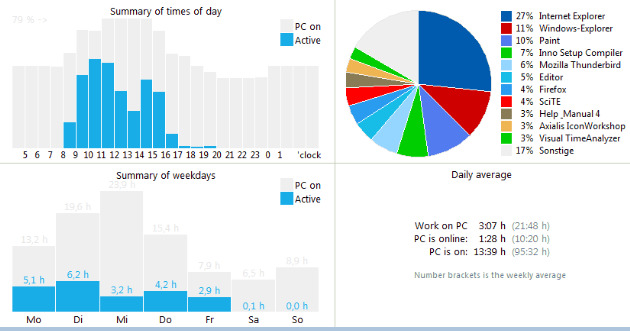
\includegraphics[width=\textwidth]{pouzitie}
	\caption{Ukážka zobrazenia štatistík ako jeden z~prípadov použitia}
\end{figure}

\newpage

\subsection{Prostredia použitia}
Program je určený najmä pre využitie v~domácom prostredí, v~prípade študentov napríklad na internáte. Je to prostredie, v~ktorom trávia väčšinu času práce na počítači. Užívateľ príde domov a po chvíli začne pracovať na počítači, môže sa jednať o~bežné činnosti, odreagovanie, štúdium z~online zdrojov, práca na školskom, pracovnom alebo osobnom projekte. Účelom aplikácie nie je monitorovanie práce v~tíme a synchronizácia medzi viacerými užívateľmi a neposkytuje ani prostriedky na pokročilú kontrolu nadriadeným, preto sa nehodí do firemného prostredia. Naopak je vhodná tam, kde užívateľ sleduje vlastné výkony a sám si plánuje svoje aktivity. Užívateľ samozrejme môže používať Time Tracker aj vo firemnom prostredí, jedná sa však len o~jeho vlastnú iniciatívu, za účelom zlepšenia sa v~rozložení práce, nie o~firemnú politiku alebo nariadenie od zamestnávateľa.

Program je desktopová aplikácia, preto sa bude používať na PC, notebookoch. Výsledné prostredie by teda byť inovatívne, jednoduché a jasné na ovládanie, no zároveň byť natívne pre daný operačný systém a prispôsobiť sa pravidlám dizajnu\cite{windows_design_guidelines} u~daného OS a neprinášať zmätočné ovládanie a prvky, na ktoré nie je bežne zvyknutý.


\begin{figure}[h!]
	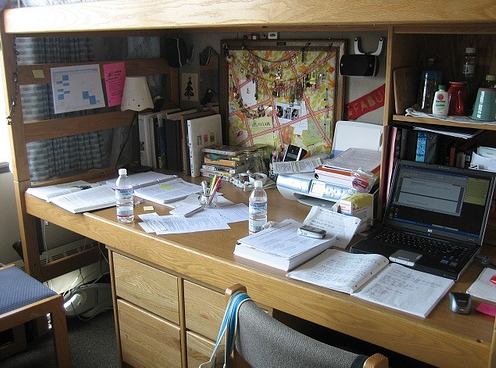
\includegraphics[width=\textwidth]{prostredie}
	\caption{Prostredie použitia}
\end{figure}

\newpage

\subsection{Požiadavky na produkt}

\begin{itemize}
	\item \textbf{problém}: užívateľ neefektívne využíva svoj čas pri činnostiach na 	počítači, vykonávanie nepovolených činností na počítači
	\item \textbf{riešenie}: program ponúka komplexný prehľad o~prebiehajúcich a vykonaných činnostiach, kategorizáciu/spoplatnenie činností, upozorňuje na nezhody s~užívateľským plánom a rovnako na nepovolené činnosti na počítači
	\item \textbf{vlastnosti a funkcie, ktoré riešia problém}: automatické zisťovanie prebiehajúcich činností, ich zaznamenávanie a prezentovanie vo forme tabuliek/grafov/zoznamov, možnosť nastavenia upozornení na nezhody v~plnení plánov, upozornenia na určité činnosti
\end{itemize}

\subsection{Existujúce riešenia}

\begin{itemize}
	\item \textbf{Toggl}\footnote{\url{https://toggl.com/}}
	\begin{itemize}
		\item[+] webová aplikácia (multiplatformová), open source, natívny klient pre Linux, jednoduché na používanie, integrácia s~existujúcimi službami, synchronizácia s~cloudom, upozornenia
		\item[--] nemožnosť porovnania odhadovanej doby s~aktuálnou, slabšia možnosť prispôsobenia farieb
	\end{itemize}
	
	\item \textbf{TimeCamp}\footnote{\url{https://www.timecamp.com/}}
	\begin{itemize}
		\item[+] webová/mobilná/desktopová aplikácia, cloud, dostupnosť bezplatnej verzie, podpora 24/7
		\item[--] chýbajúca možnosť upozornia o~používaní sociálnych sietí, zložitá navigácia, staršie rozhranie
	\end{itemize}
	
	\item \textbf{Project Hamster}\footnote{\url{https://projecthamster.wordpress.com/}}
	\begin{itemize}
		\item[+] sledovanie projektov, pridávanie značiek k~činnostiam, prehľad za časové obdobia, generovanie dát o~činnostiach vhodných na tlač, dlhodobá podporu
		\item[--] chýbajúce automatické zaznamenávanie aktivít, podpora len Gnome 3
	\end{itemize}

\end{itemize}

\newpage

\section{Návrh kľúčových prvkov UI}
Program bude používaný na počítači, preto je nutné sa zamerať na interakciu pomocou myši a klávesnice. Používateľovi taktiež musí byť jasné, ako sa program ovláda, kde nájde pomocníka, kde nastavenia, a pod. Upozornenia programu by mali byť jasné a zrozumiteľné.

Používateľ bude môcť používať automatickú detekciu prebiehajúcich činností, ktorú ponúka program. Alternatívne si bude môcť spustiť/pozastaviť/zastaviť činnosť, ktorú chce sledovať.
Samotný program bude obsahovať zoznamy - zoznam činností a kategórie činností. Položky v~týchto zoznamoch musia obsahovať potrebné informácie o~činnosti - dobu trvania, názov činnosti ale aj možnosti na správu činnosti - premenovať, zmazať, zmeniť údaje, a pod. 

Program bude poskytovať možnosť zobrazenie prehľad o~činnostiach za zvolené časové obdobie vo forme tabuliek, grafov, z~možnosťou ich uloženia. Taktiež bude dostupné menšie okno na manuálne spustenie sledovania činností. Upozornenia z~programu budú využívať natívne riešenie pre zobrazenie upozornení na danom systéme a budú používateľa informovať o~činnostiach, prípadne o~nesúľade vytvoreného plánu činností so skutočnosťou.

\subsection{Návrh GUI a prototyp}

\begin{figure}[h!]
	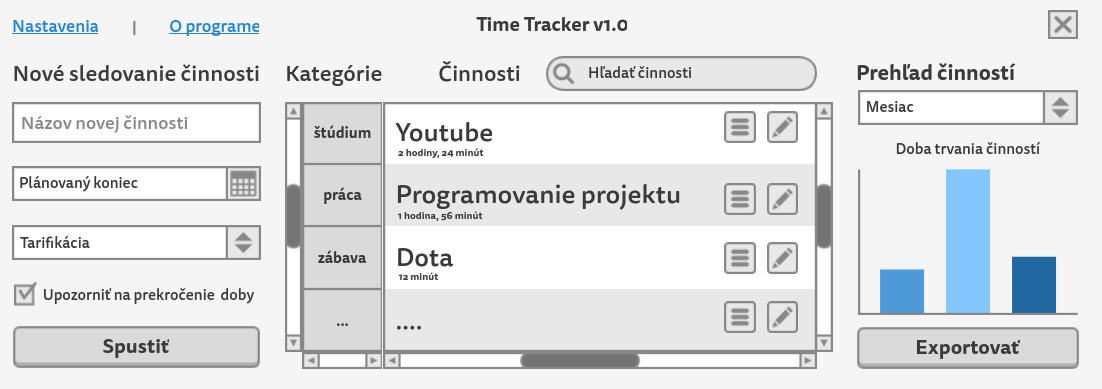
\includegraphics[width=\textwidth]{prototyp}
	\caption{Prototyp programu}
\end{figure}

Prototyp sa zameria na program, ktorý podľa návrhu hneď z~hlavného okna bude umožňovať manuálne spustenie sledovania činnosti, zobrazenie zoznamu činností/kategírií činností, vyhľadávanie v~činnostiach. Pri každej činnosti je uvedený čas ako dlho prebieha a tlačidlá na správu danej činnosti. Program v~hlavnom okne taktiež bude ponúkať možnosť zobrazenia prehľadu o~vykonaných činnostiach za určité časové obdobie.

\section{Testovanie prototypu GUI}

Vytvorený prototyp GUI bol podrobený testovaniu. Táto kapitola popisuje spôsob testovania, vyhodnotenie a záver z~výsledkov testovania.

\subsection{Individuálny návrh testovania}
Testovací protokol má podobu online dotazníka\cite{vyhodnotenie} otvorených aj uzavretých otázok. Online dotazník považujeme za jednoduchý spôsob ako získať odpovede na otázky a pre užívateľov je vyplnenie dotazníka nenáročná, párminútová zaležitosť. Je dôležitá správna formulácia otázok a identifikácia závislostí\cite{experimenty}.

V~dotazníku sa nachádzajú otázky všeobecného charakteru -- pohlavie, vek a následne otázky špecifické pre Time Tracker. V~mojom navrhnutom dotazníku som zisťoval, aké sú znalosti ľudí o~programoch ako je Time Tracker. Ďalej ma zaujímalo prostredie, kde by sa program používal.  V~nasledujúcej otázky som zisťoval, aké operačné systémy respondenti používajú, a teda, na ktorých by spúšťali Time Tracker. Dôležitým faktorom ovplyvnujúcim spokojnosť so softvérom je aj jazyk softvéru -- pýtal som sa na preferovanú lokalizáciu programu. Ďalšie otázky sa týkali vlastností Time Trackera, ktoré užívatelia považujú za najdôležitejšie. Následne sa prezentoval prvotný návrh GUI a reakcie užívateľov na tento návrh – plus, mínusy, návrhy na zlepšenia, atď.

Dotazník poskytol prehľadné výsledky o~preferenciách užívateľov a otázky s~otvorenou odpoveďou priniesli nové nápady, inšpirácie, návrhy na zmeny a vylepšenia. Spätná väzba k~prvotnému návrhu poskytuje cenné informácie do budúceho vývoja grafického rozhrania.

\subsection{Výsledný testovací protokol}
Finálna forma dotazníka obsahovala nasledovné otázky:

\begin{enumerate}
	\item Pohlavie
	\item Veková skupina (menej ako 18, 18-44, 44-60, 60 a viac)
	\item V~akom prostredí by ste chceli používať Time Tracker? (doma, v~práci, v~škole, iné)
	\item Aký operačný systém používate? (Linux, Windows, Mac OS, iné)
	\item Za akým účelom by ste Time Tracker používali? (sledovanie činností, plánovanie činností, obmedzenie činností, výpis štatistík, kontrola činností na PC)
	\item Poznáte programy typu Time Tracker?  
	\item Ktoré vlastnosti Time Trackeru považuje za najdôležitejšie? (sledovanie činností, plánovanie aktivít , upozornenia na prekročenie času, kategorizácia činností, multiplatformovosť, výpočet odmien, kontrola činností, zobrazenie štatistík)
	\item Aký jazyk programu preferujete? (angličtina, slovenčina, čeština,iné)
	\item Uvítali by ste možnosť ovládať sledovanie času pomocou klávesových skratiek?
	\item Akým spôsobom by vás program upozorniť na prekročenie času činnosti? (vyskakovacie okno, zvuk, e-mail, iné)\\
	
	\textit{Nasleduje snímka obrazovky prototypu GUI (hlavné okno)}
	\begin{figure}[h!]
		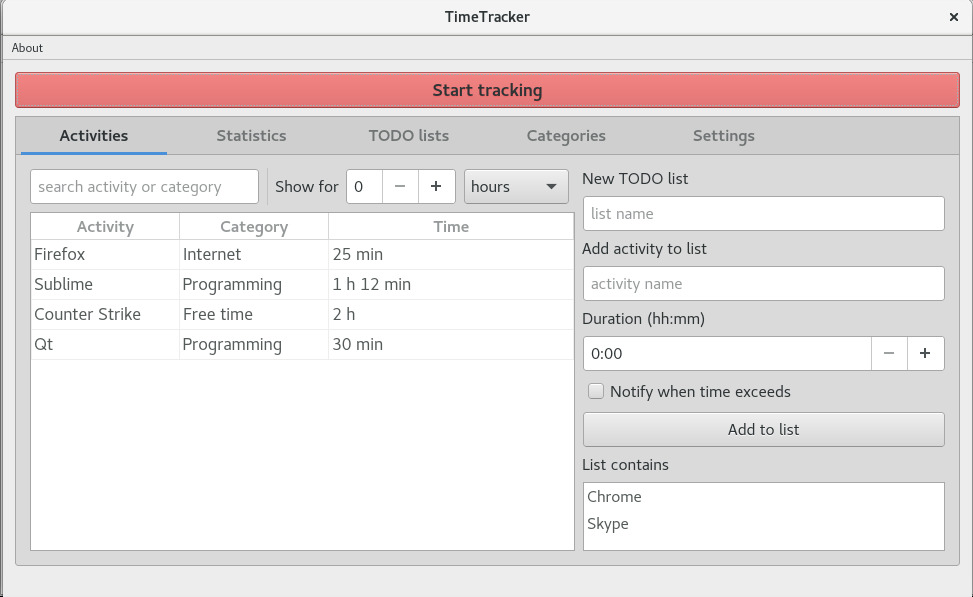
\includegraphics[width=\textwidth]{hlavna_obrazovka}
		\caption{Hlavná obrazovka programu}
	\end{figure}
	\item Ktoré tvrdenia vystihujú hlavné okno programu? (vhodné rozloženie prvkov, prehľadné zobrazenie, jasná funkcionalita, jednoduché ovládanie, neprehľadnosť)
	\item Váš prvý dojem z~programu
	\item Čo by ste na rozhraní zmenili? 
\end{enumerate}

\subsection{Realizácia testov}
Oslovil som svoj okruh kamarátov, známych a požiadal som ich o~vyplnenie online dotazníka. 

\subsection{Výsledky a závery}

Odpovede z~dotazníku sme vyhodnotili a následne sme vytvorili záver z~testovania, ktorý ovplyvnil ďalší vývoj programu.

\subsubsection{Vyhodnotenie dotazníka}

Dotazník bol prístupný na Formulách Google\footnote{\url{https://www.google.com/intl/sk/forms/about/}}, kde prebiehalo samotné vypĺňanie dotazníka. Oslovili sme ľudí z~nášho okolia, a teda sa jednalo prevažne o~študentov študujúcich FIT VUT v~rôznych ročníkoch. Pomocou dotazníka sme získali 66 odpovedí. Odpovede na otázky su uvedené v~kapitole \ref{literatura} -- Prílohy. Prevahu v~pohlaví mali muži nad ženami. Absolútna väčšina respondentov sa zaradila do vekovej kategórie 18-44 rokov. Otázka na prostredie potvrdila naše predpoklady na cieľové prostredie na prácu s~Time Trackerom, keďže väčšina respondentov preferovala domáce, prípadne pracovné prostredie. V~otázke ohľadom používaného operačné systému sa nám potvrdilo správnosť prvotného rozhodnutia o~multiplatformové riešenie nášho programu – z~výsledkov je jasné, že Windows a Linux sú najpoužívanejšie OS u~našich respondentov. V~ďalšej otázke nás zaujímalo, za akým učelom by respondenti Time Tracker využívalo. Z~výsledkov vyplynulo, že by šlo prevažne o~sledovanie aktivít na PC ale aj ich plánovanie do budúcnosti. Z~dotazníku taktiež  poznať, že nadpolovičná väčšina respondentov Time Tracker nepoužíva, čo sa ale aj očakávalo kvôli špecifickému charakteru a poskytovaným funkciám takého typu softvéru. Ako jazyk programu je podľa odpovedí preferovaný anglický jazyk, no taktiež sú žiadané lokálne jazyky ako je čeština a slovenčina. Respondenti taktiež prejavili záujem o~možnosť ovládania programu pomocou kláves/klávesových skratiek. Ďalej nás zaujímalo, aké formy upozorňovania by mal program používať – podľa výsledkov najžiadanejšími formami by boli vyskakovacie upozornenia a upozornenia zvukom.

Následne sme poskytli respondentom snímku obrazovky prototypu GUI a ďalšie otázky sa venovali práve tomuto prototypu. Vlastností, ktoré vystihujú hlavné okno programu sú prevažne prehľadnosť rozhrania, vhodné rozloženie prvkov rozhrania a taktiež ovládanie programu považovali za jasné. Posledná otázka bola s~otvorenou formou odpovede a smerovala na názor respondenta na tento prototyp. Z~poskytnutej spätnej väzby je zrejmé, že je potrebné zjednodušiť hlavné okno týkajúce sa zobrazenia činností, pridať miernu farebnosť do rozhrania, zmeniť popis niektorých častí rozhrania programu pre jednoduchšiu orientáciu a ovládanie programu.

\subsubsection{Záver z~testovania a dopad na navrhnuté GUI}

Po vyhodnotení otázok vyplynulo, že respondenti by uvítali podporu viacerých jazykov programu, konkrétne angličtiny, slovenčiny, češtiny, ktoré budú pridané do programu. Taktiež vyplynulo, že podpora klávesových skratiek by bola vo veľkej miere vítaná, túto funkcionalitu do programu taktiež pridáme. Z~odpovedí o~použití operačného systému sa nám potvrdil záujem o~multiplatformnosť (viď. Qt\cite{doc_qt}), keďže najviac užívateľov používa Windows a Linux. Respondenti najviac požadovali upozornenia vyskakovacím oknom a zvukom, tieto 2 spôsoby zapracujeme do programu. Pre užívateľov sú z~hľadiska funkcionality najviac podstatné funkcie sledovania času, plánovania aktivít a zobrazenia štatistík, čomu prispôsobíme aj užívateľské rozhranie. Do dotazníku sme pridali návrh hlavného okna programu, z~individuálnych odpovedí vyplynulo, že užívateľom nevyhovuje vytvorenie nového TODO listu na hlavnej obrazovke. Vytvorenie presunieme do inej logickej časti týkajúcej sa len TODO listov. Rovnako by uvítali v~GUI viac farieb, najmä zmenu farby tlačidla na spustenie sledovania. 

\section{Implementácia}

Obsahom tejto kapitoly sú implementačné záležitosti ohľadne voľby technológií na tvorbu programu a vývoja backendu a fronendu. Kapitola obsahuje aj snímky obrazovky finálne grafického rozhrania s~popisom jednotlivých častí programu. 

\subsection{Výber technológií}
Náš program sme sa rozhodli vyvíjať pre operačné systémy Linux a Windows ako klasickú desktopový program. Z~dotazníka vyplynulo, že najväčší počet respondentov používa tieto dva  systémy a program nájde svojich potencionálnych užívateľov na obidvoch platformách. Program je plne funkčne pripravený pre systém Linux, pre Windows však v~tomto čase ešte nie je funkčné sledovanie spustených programov.

Na tvorbu GUI a backendu sme si zvolili multiplatformný framework Qt\cite{doc_qt}. Táto možnosť nám prišla ako najlepšia voľba, pretože Qt poskytuje množstvo funkcií a prvkov na tvorbu GUI a back-endu pre desktopové programy. Pri tvorbe GUI sme využili aj rozšírenie QML\cite{qml}, ktoré umožňuje návrh pokročilejších grafických prvkov pre GUI, ktoré je možné použiť spoločne s~prvkami vytvorenými len pomocou Qt bez QML. Ďalšou výhodou Qt bolo použitie jazyka C++\footnote{\url{www.cplusplus.com}} na tvorbu grafických prvkov ako aj funkcionality, pretože s~ním už máme všetci skúsenosti.
Framework Qt nám značne uľahčil návrh a tvorbu grafických prvkov rozhrania. Pomocou QML sme boli schopní navrhnúť hlavné menu programu. Zvyšné časti sme tvorili len pomocou grafických prvkov, ktoré Qt poskytuje.

\subsection{Backend}
Hlavnou funkciou programu je automatické sledovanie spustených programov na počítači a ich čas behu. Sledovanie aktívnych programov prebieha každú sekundu, aby mal užívateľ vždy aktuálne údaje. Automatické sledovanie je možné vypnúť, v~tom prípade je nutné zahájiť sledovanie manuálne. Sledovanie je možné kedykoľvek pozastaviť a znovu obnoviť.
Medzi ďaľšie dôležité funkcie programu patria vytváranie vlastných TODO listov a ich správa, vytváranie vlastných kategórií pre programy a zobrazovanie štatistík programov.

Program poskytuje užívateľom pri práci s~TODO listami funkcie vytvorenia nového listu a aktivít listu, odstránenie listu alebo aktivity, premenovanie listu. Na odstraňovanie a premenovanie listu ako aj aktivít v~liste je možné využiť klávesové skratky, ktoré užívatelia požadovali v~rámci testovania. Do vytvoreného listu môže užívateľ pridať aktivitu s~dobou trvania alebo ju z~listu odstrániť. Dôležitou funkciou je sledovanie zvoleného listu, po ukončení trvania všetkých jeho aktivít je možné užívateľa upozorniť na jeho ukončenie. V~nastaveniach programu môže užívateľ zvoliť či chce byť upozorňovaný a akým spôsobom sa to má uskutočniť. Na výber má možnosť vyskakovacieho okna a zvuku.

V~rámci práce s~kategóriami môže poskytuje program užívateľovi funkcie vytvorenia novej kategórie, odstránenie a premenovanie kategórie. Do vytvorenej kategórie je možné pridať program alebo ju odobrať. Pre každú činnosť je v~rámci GUI vytvorené tlačidlo na realizáciu danej funkcie. Premenovanie sa realizuje pomocou dvojkliku na meno kategórie, po ktorom sa zobrazí dialógové okno, kde sa zadá nový názov. Ďalšou možnosťou je využitie klávesovej skratky. Odstraňovanie je možné pomocou tlačidiel alebo klávesovou skratkou.

Štatistiky poskytujú užívateľovi prehľad o~spustených programoch spolu s~priradenou kategóriou, trvaním a počtom spustení. Na zobrazenie údajov sme použili aj formu grafov, ktoré zobrazujú údaje o~časoch jednotlivých programov a časovom zábere jednotlivých kategórií. Funkcia výpočtu peňažnej hodnoty za použitie nejakého programu je implementovaná vo forme jednoduchej kalkulačky, ktorá dostane na vstup názov aktivity a vypočíta hodnotu za dobu trvania aktivity

Program poskytuje užívateľom možnosť prispôsobiť si určité vlastnosti programu v~rámci Nastavení. Užívateľ má možnosť zvoliť veľkosť písma na hlavnej obrazovke, vypnúť automatické sledovanie, zvoliť si upozornenia, ich spôsob, trvanie a nakoniec možnosť skryť prítomnosť kalkulačky v~zobrazení. V~rámci obrazovky nastavení sú vysvetlené klávesové skratky programu. 

\subsection{Frontend}
Grafické rozhranie sme implementovali pomocou Qt a QML. Program sme logicky rozdelili na 5 samostatných okien, podľa zvolenej položky v~menu sa zobrazí okno s~príslušnými funkčnými prvkami. Každé okno zobrazuje iné prvky týkajúce sa danej funkcionality programu. Menu programu sme vytvorili pomocou QML. Pri tvorbe GUI nám pomohla spätná väzba z~dotazníka, kde bol dostupný mockup obrazovky programu. Užívatelia si žiadali pridať viac farieb a sprehľadniť hlavnú obrazovku. Tieto poznatky sme zakomponovali do finálnej podoby GUI. Pri návrhu farieb sme sa tiež riadili odporúčaniami z~pravidiel dizajnu pre Material Design\cite{material_design_guidelines}.

\newpage

Hlavné okno programu je tvorené panelom menu na ľavej strane a jedným z~5 okien na pravej strane. V~hornej časti sa nachádza tlačidlo na ovládanie spúšťania a zastavovania sledovania aktivít.

\begin{figure}[h!]
	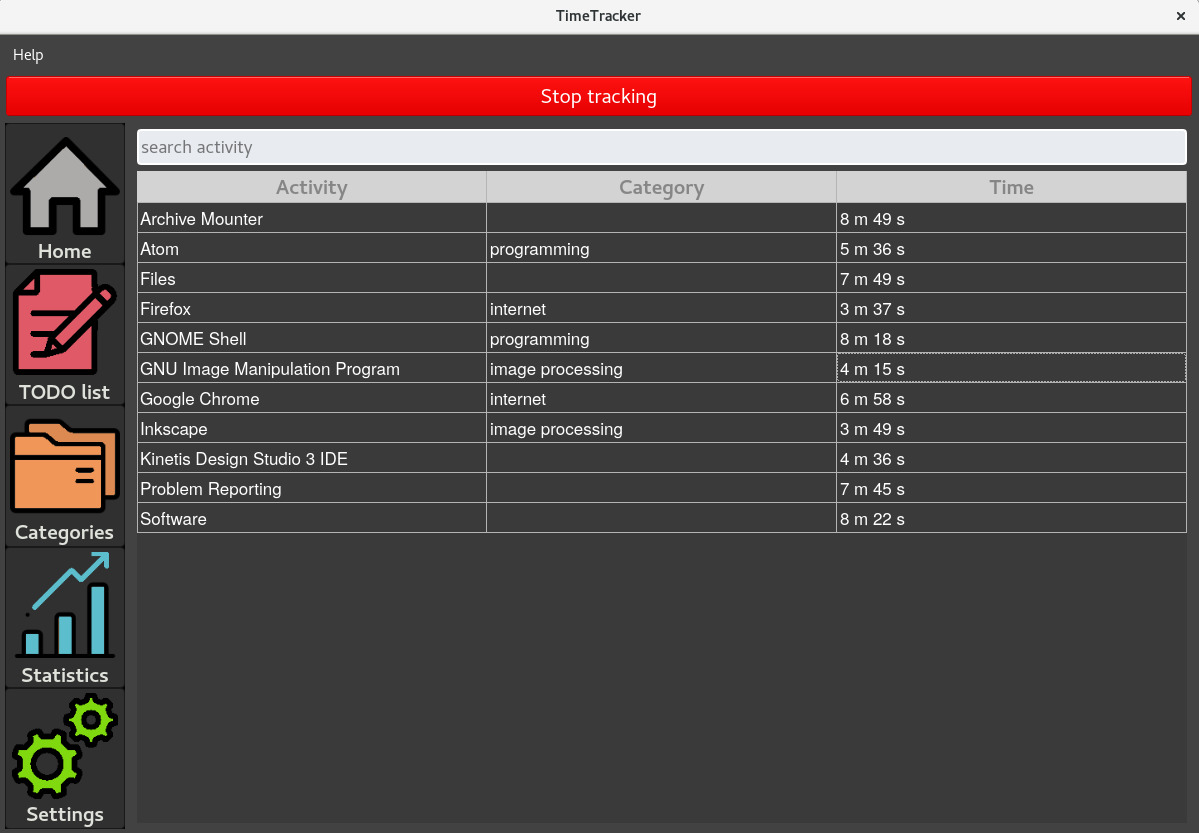
\includegraphics[width=\textwidth]{domaca_obrazovka}
	\caption{Domáca obrazovka programu}
\end{figure}

Domáca obrazovka programu obsahuje tabuľku s~prehľadom o~aktivitách a panel na vyhľadávanie v~nej. Ak užívateľ zadá slovo do vyhľadávania, riadok tabuľky, ktorý slovo obsahuje je zvýraznený farbou zvolenou užívateľom v~Nastaveniach. Po pripomienkach z~dotazníka sme z~tohto okna odstránili vytváranie TODO listu.

\newpage
\begin{figure}[h!]
	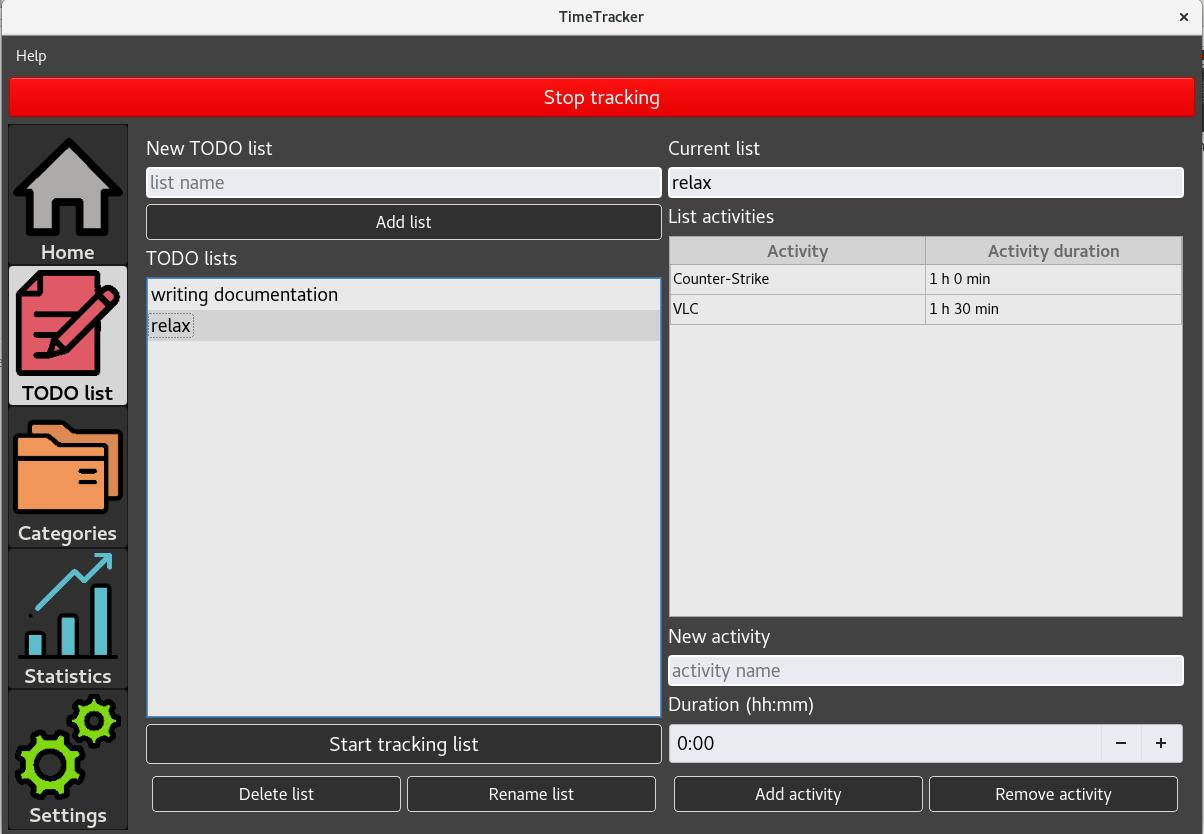
\includegraphics[width=\textwidth]{todo_listy}
	\caption{TODO listy}
\end{figure}

V~ľavej časti obrazovky môže užívateľ vytvárať nový list, odstraňovať list. Zobrazovanie aktuálnych listov je vo forme listu s~menami. Užívateľ má poskytnuté tlačidlá na vytvorenie listu, odstránenie listu a začatie sledovania. Po začatí sledovania sa v~spodnej časti okna zobrazí tabuľka s~aktuálnymi aktivitami sledovaného listu a ich trvaním. Po dokončení listu tabuľka zmizne. 

Pravá časť obrazovky slúži na pridávanie aktivít do listu a odstraňovanie z~listu. Takisto sa v~tejto časti zobrazujú aktivity vybraného TODO listu.

\newpage

\begin{figure}[h!]
	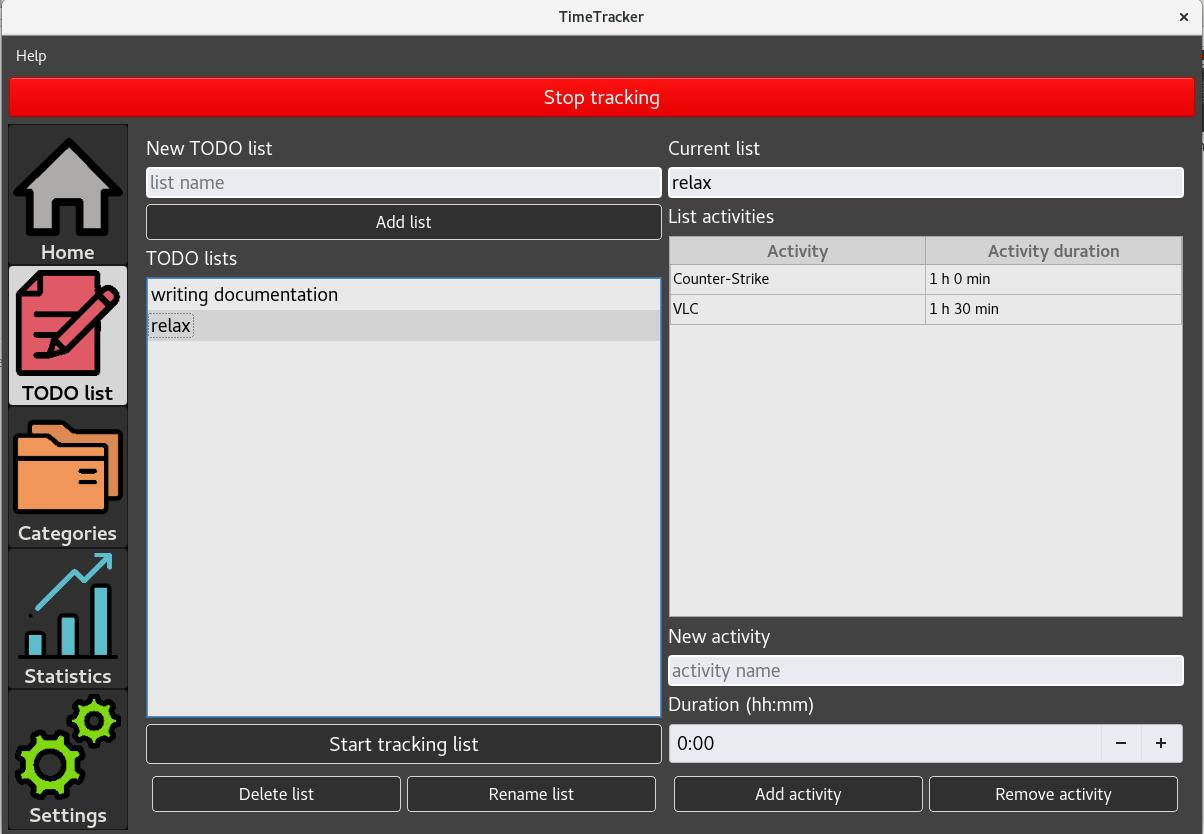
\includegraphics[width=\textwidth]{todo_listy}
	\caption{Kategórie}
\end{figure}

Obrazovka pre kategórie je podobne ako u~TODO listov rozdelená na 2 logické časti. V~ľavej časti sa vytvárajú, odstraňujú a zobrazujú kategórie. V~pravej časti sa vytvárajú, odstraňujú a zobrazujú položky zvolenej kategórie. Užívateľ môže na odstraňovanie kategórie a položky kategórie využiť tlačidlo alebo klávesovú skratku.

\newpage

\begin{figure}[h!]
	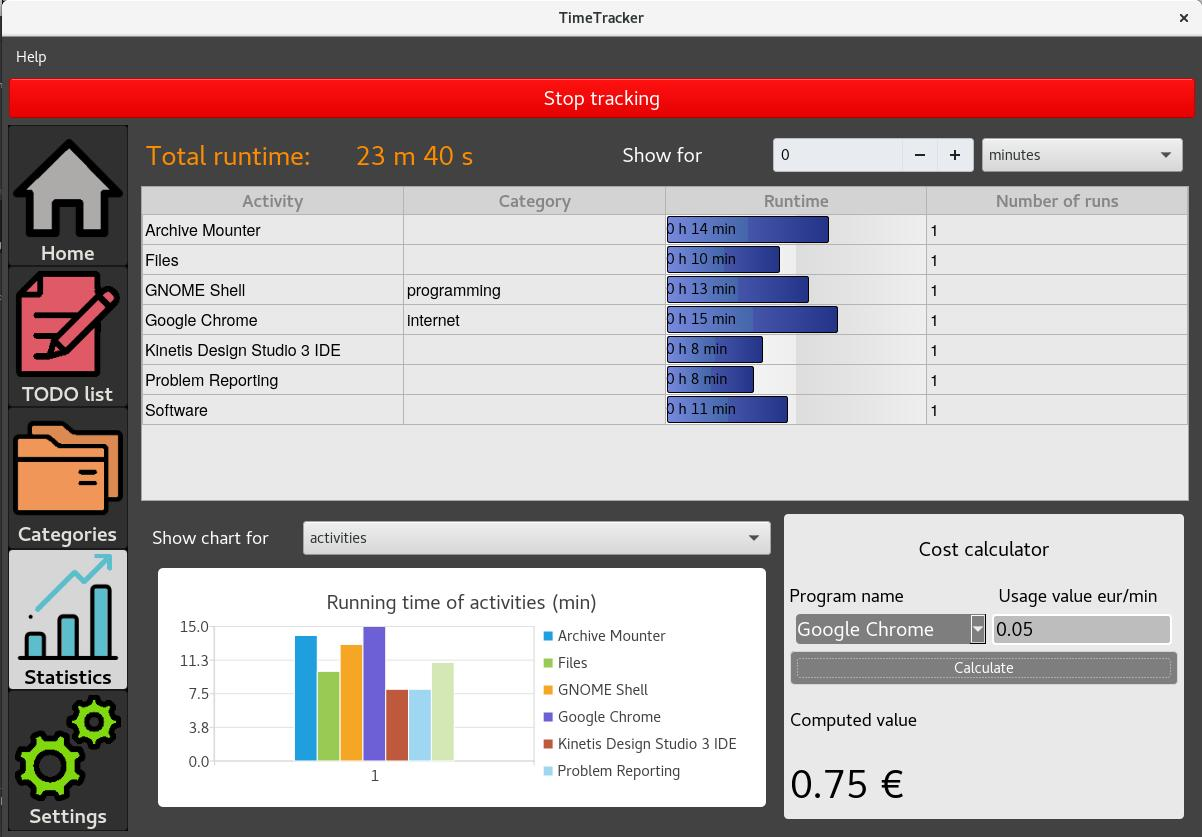
\includegraphics[width=\textwidth]{statistiky}
	\caption{Štatistiky}
\end{figure}

Obrazovka so štatistkami je rozdelená na hornú a dolnú časť. V~hornej časti sa zobrazujú informácie o~čase behu programu a jednotlivých bežiacich aktivitách. Aktuálne bežiace programy sú zobrazené v~tabuľke s~informáciami o~kategórií, čase behu aktivity a počte behov aktivity. U~behu aktivity je použitý panel o~prebehu na vyjadrenie časti, ktorú zaberá beh aktivity z~celkového behu TimeTrackeru. Položky v~tabuľke sa zobrazujú podľa zvoleného času trvania, ktoré môže užívateľ zvoliť pomocou tlačidiel v~pravej časti.

Spodná časť slúži na zobrazenie grafov, ktoré prezentujú získané údaje. Užívateľ si môže pomocou tlačidla zvoliť zobrazenie grafu aktivít alebo kategórií. Nachádza sa tu aj kalkulačka na výpočet ceny za použitie zvoleného programu. Tento prvok je možné odstrániť z~viditeľnej časti pomocou nastavenia v~Nastaveniach.

\newpage

\begin{figure}[h!]
	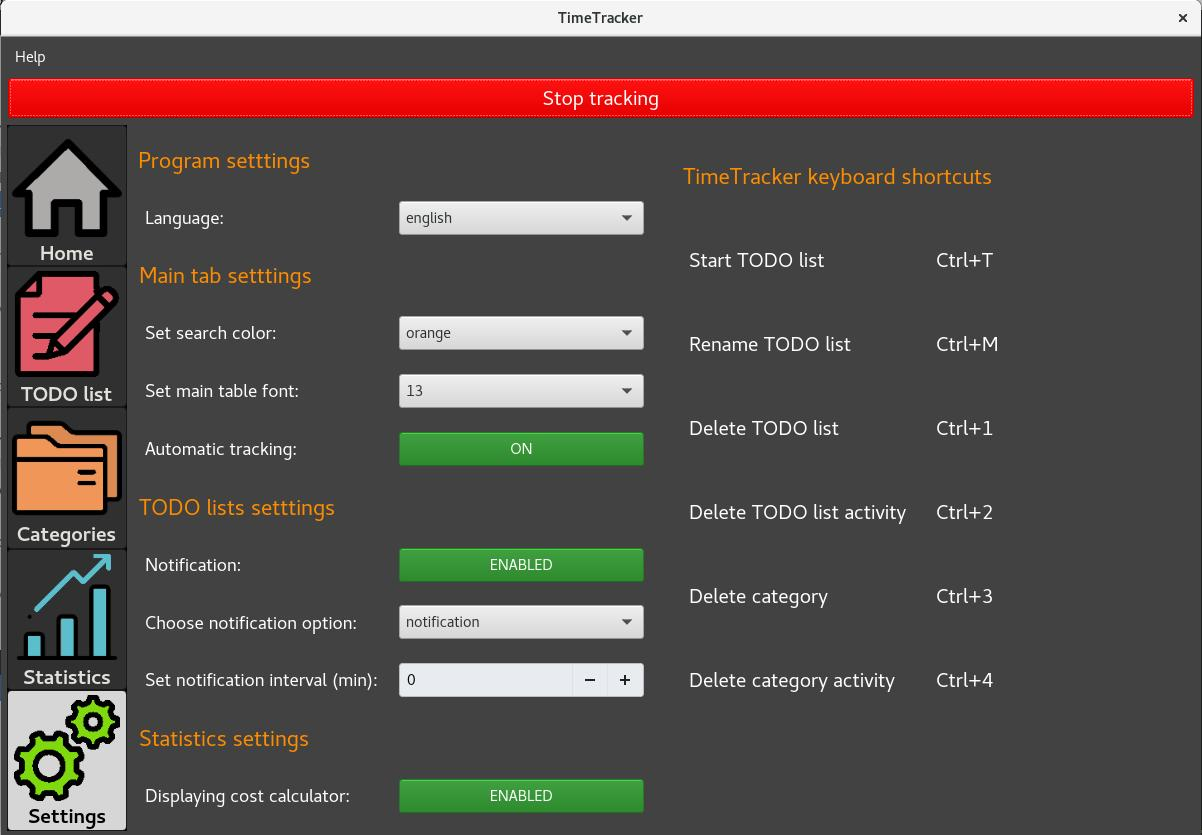
\includegraphics[width=\textwidth]{nastavenia}
	\caption{Nastavenia}
\end{figure}

Poslednou obrazovkou programu je zobrazenie Nastavení. Obrazovka má opäť 2 časti, ľavá časť zobrazuje nastavenia pre jednotlivé obrazovky, pravá časť zobrazuje vysvetlenie klávesových skratiek programu.

\newpage

\section{Užívateľské testovanie}

Testovaným subjektom (ďalej ako \uv{užívatelia}) sme zadali zoznam úlohy ktoré majú vykonať, pozorovanie bolo priame\cite{vyhodnotenie}. Sledovali to ako si s~úlohou poradia, ako dlho im to trvá, aký postup zvolili pre splnenie úlohy. Užívatelia nahlas komentovali kroky k~vyriešeniu úlohy a ich myšlienkové pochody, jednalo sa teda o~protokol hlasného myslenia\cite{vyhodnotenie}. Zadané úlohy sú popísane v~kapitole \ref{ulohy}. Testovania sa zúčastnili 4 osoby, jednalo sa o~študentov VŠ, vo veku od 19 do 24 (1 žena, 3 muži). Testovanie užívateľov bolo oddelené, každý z~nich mal vykonať rovnakú sadu úloh. Testovanie bolo uskutočnené v~záverečných fázach vývoja produktu. 

\subsection{Úlohy a výsledky}
\label{ulohy}

\begin{itemize}
	\item \textbf{Zistite aktuálne bežiace programy a čas ich behu}
	
	 Užívatelia s~úlohou problém nemali, užívatelia sa v~rozhraní zorientovali pomerne rýchlo a nebolo pre nich následne náročne nájsť požadované informácie.
	
	\item \textbf{Medzi bežiacimi programami vyhľadajte tie, ktoré v~názve obsahujú „w“}
	
	Užívatelia boli schopní nájsť prvok slúžiaci na vyhľadávanie. Niektorým užívateľom nebolo jasné ako vyhľadávanie funguje. Po zadaní textu čakali, že sa ihneď nájdu požadované programy. Niektorí z~nich došli k~správnemu riešeniu úlohy, ktorý spočíva v~zadaní textu do prvku a stlačením klávesy „Enter“, avšak chvíľu im to trvalo a klávesu nestlačili okamžite. Počas plnenia úlohy spozorovali príliš dlhý čas od spustenia vyhľadávania po zmenu v~rozhraní.
	
	Na základe výsledkov testovania z~tejto úlohy sme sa rozhodli, zobrazovať priebežný výsledok vyhľadávania ihneď pri jeho zadávaní do vyhľadávacieho poľa. Taktiež sme znížili čas potrebný na zmeny rozhrania spôsobenú vyhľadávaním, ktorá bola predtým riadená intervalom prekresľovania tabuľky, po úprave dochádza k~zobrazeniu výsledku takmer okamžite a nečaká sa na prekreslenie tabuľky.
	
	\item \textbf{Vytvorte nový TODO list a pridajte do neho dve aktivity}
	
	Užívatelia našli bezproblémovo položku pre TODO listy v~hlavnom menu, taktiež im nerobilo problém vytvoriť nový TODO list. V~pravej časti okna našli tabuľku obsahujúci aktivity pre daný TODO list, následne im nerobilo problém pomocou pridať novú aktivitu do zoznamu.
	
	\item \textbf{Premenujte vytvorený TODO list}
	
	S~touto úlohou mali užívatelia najväčšie problémy, nevedeli akým spôsobom majú úlohu vykonať. Premenovanie TODO listu bolo pôvodne realizované prostredníctvom dvojkliku na jeho názov. Tento postup žiadneho z~užívateľov nenapadol. Preto sme sa rozhodli pridať ďalšie tlačidlo, ktoré je určené na premenovanie TODO listu. Keďže sme podobný prístup volili aj pri premenovaní kategórií, podobnú zmenu sme vykonali aj tam.
	
	\item \textbf{Zobrazte graf pre kategórie}
	
	Obrázok v~hlavnom menu užívateľom napovedal, kde potrebný graf nájdu. Užívatelia nemali problém zo zobrazením štatistík a taktiež takmer hneď našli prvok slúžiaci na výber grafu, ktorý sa má zobraziť. Pomocou prvku následne správne zvolili graf pre kategórie.
	
	\item \textbf{V~štatistikách vyrátajte sumu za použitie ľubovoľného programu a poplatok za používanie nastavte na 0.05 eur za minútu}
	
	Užívatelia v~štatistikách našli kalkulačku určenú na vykonanie tejto úlohy a následne aj prvky na výber programu, zadanie poplatku. Následný výpočet na získanie sumy im nerobil žiadny problém.
	
	\item \textbf{Zmeňte spôsob upozornení na kombinované upozornenie zvukom a notifikačnou správou}
	
	Užívatelia ihneď zvolili správny postup -- prechod do nastavení, kde našli položku, ktorá mení spôsob upozornenia. U~všetkých užívateľov bolo vykonanie tejto úlohy bezproblémové.
	
	
\end{itemize}

\newpage

\section{Záver}

\subsection{Tímová spolupráca}
Program sme vytvárali v~tíme. Prínosom takejto spolupráce bolo viac pohľadov na problémy. Pri tvorbe testovacieho dotazníka každý člen pridal svoje myšlienky a nápady na otázky. Takisto nám viac pohľadov pomohlo pri tvorbe GUI a ladení rôznych prvkov a farieb. Dôležitá bola komunikácia v~tíme. 

Implementácia backend a frontend častí programu bola rovnomerne rozložená medzi všetkých členov tímu s~cieľom odskúšať si zvolené technológie a postupy tvorenia GUI.

\subsection{Výsledný program}
Na základe prvotného prototypu a spätnej väzby na GUI programu sme implementovali finálnu podobu našeho programu. Odporúčania opýtaných respondentov nám pomohli značne vylepšiť vzhľad programu.

Vo finálnej podobe umožňuje Time Tracker sledovanie bežiacich programov, vytváranie a sledovanie vlastných TODO listov, priraďovať užívateľom vytvorené kategórie ku programom, zobrazovať štatistiky bežiacich programov. Na základe odpovedí od respondentov sme implementovali aj rôzne požadované funkcie ako napríklad ovládanie určitých funkcií pomocou klávesových skratiek.

\newpage

\section{Študijné zdroje}
\label{literatura}
\begin{thebibliography}{3}
	\bibitem{vyhodnotenie} 
	Vítězslav Beran:
	\textit{Vyhodnocení uživatelského rozhraní}.\\
	\url{https://www.fit.vutbr.cz/study/courses/ITU/private/labs/design/itu-vyhodnoceni-poznamky.pdf}
	
	\bibitem{experimenty} 
	Vítězslav Beran:
	\textit{Experimenty a vyhodnocení rozhraní}.\\
	\url{https://www.fit.vutbr.cz/study/courses/ITU/private/labs/design/itu-evaluace.pdf}
	
	\bibitem{windows_design_guidelines} 
	Windows Design Guidelines\\
	\url{https://msdn.microsoft.com/en-us/library/windows/desktop/dn688964(v=vs.85).aspx}
	
	\bibitem{doc_qt} 
	Framework Qt\\
	\url{http://doc.qt.io/}
	
	\bibitem{qml} 
	Qt QML\\
	\url{http://doc.qt.io/qt-5/qtqml-index.html}
	
	\bibitem{material_design_guidelines} 
	Material Design Guidelines\\
	\url{https://material.io/guidelines/}
\end{thebibliography}

\newpage

\section{Prílohy}

\begin{figure}[h!]
	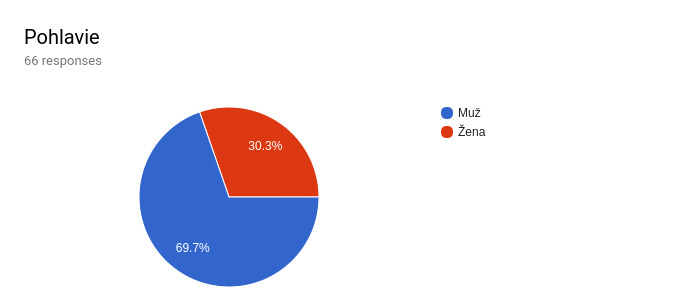
\includegraphics[width=\textwidth]{otazka1}
	\caption{Výsledky otázky č. 1}
\end{figure}

\begin{figure}[h!]
	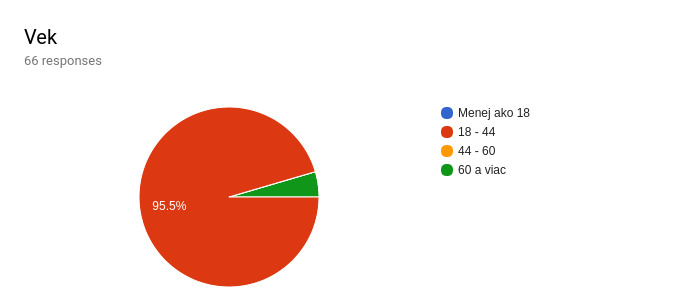
\includegraphics[width=\textwidth]{otazka2}
	\caption{Výsledky otázky č. 2}
\end{figure}

\begin{figure}[h!]
	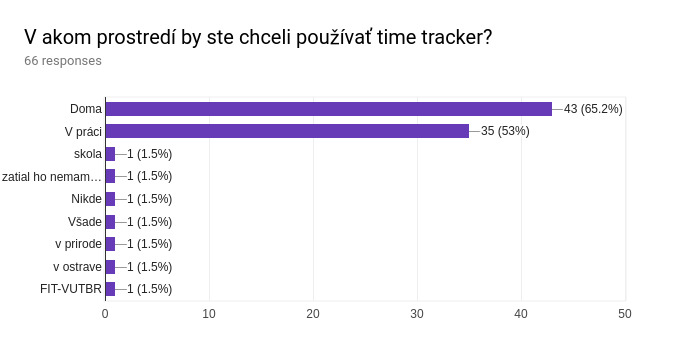
\includegraphics[width=\textwidth]{otazka3}
	\caption{Výsledky otázky č. 3}
\end{figure}

\begin{figure}[h!]
	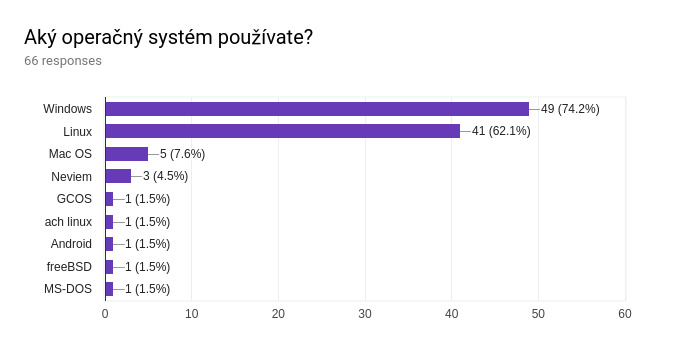
\includegraphics[width=\textwidth]{otazka4}
	\caption{Výsledky otázky č. 4}
\end{figure}

\begin{figure}[h!]
	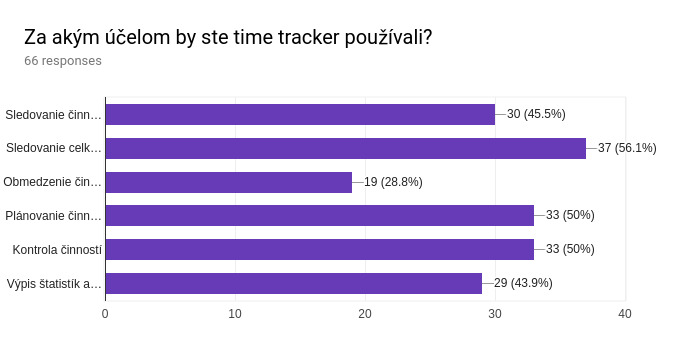
\includegraphics[width=\textwidth]{otazka5}
	\caption{Výsledky otázky č. 5}
\end{figure}

\begin{figure}[h!]
	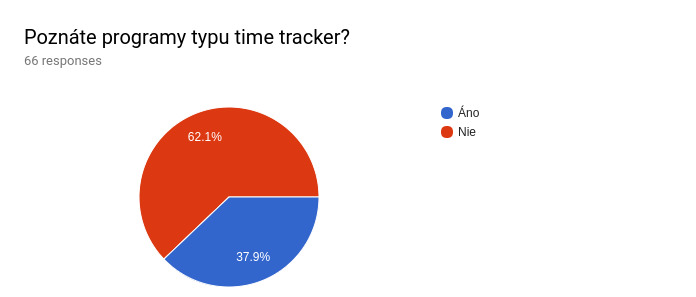
\includegraphics[width=\textwidth]{otazka6}
	\caption{Výsledky otázky č. 6}
\end{figure}

\begin{figure}[h!]
	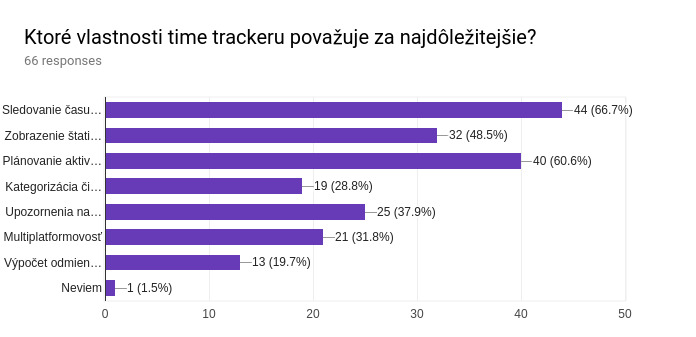
\includegraphics[width=\textwidth]{otazka7}
	\caption{Výsledky otázky č. 7}
\end{figure}

\begin{figure}[h!]
	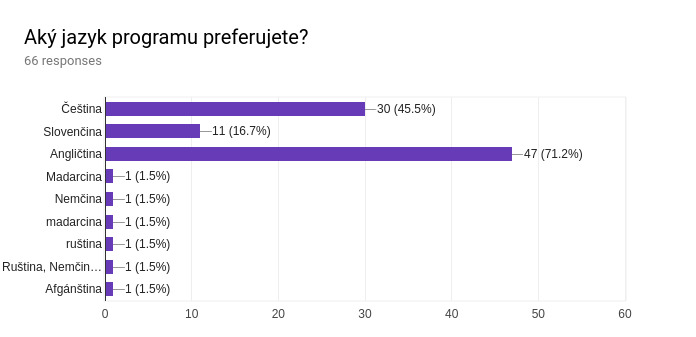
\includegraphics[width=\textwidth]{otazka8}
	\caption{Výsledky otázky č. 8}
\end{figure}

\begin{figure}[h!]
	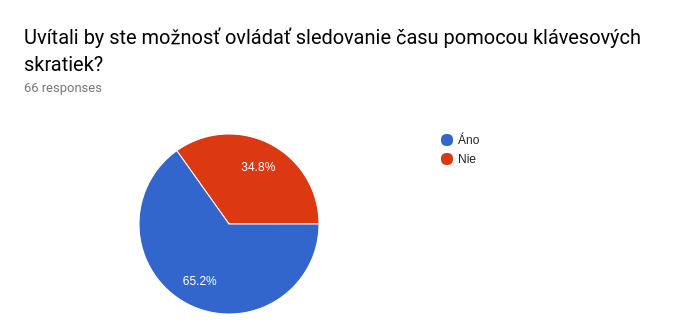
\includegraphics[width=\textwidth]{otazka9}
	\caption{Výsledky otázky č. 9}
\end{figure}

\begin{figure}[h!]
	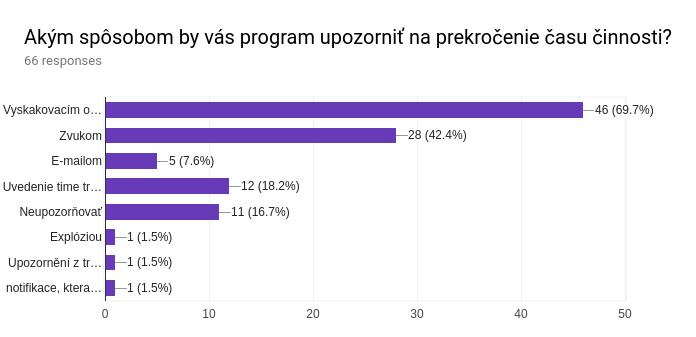
\includegraphics[width=\textwidth]{otazka10}
	\caption{Výsledky otázky č. 10}
\end{figure}

\begin{figure}[h!]
	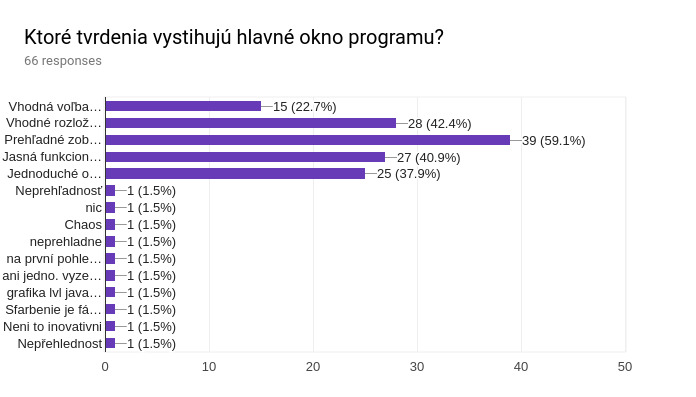
\includegraphics[width=\textwidth]{otazka11}
	\caption{Výsledky otázky č. 11}
\end{figure}

\begin{figure}[h!]
	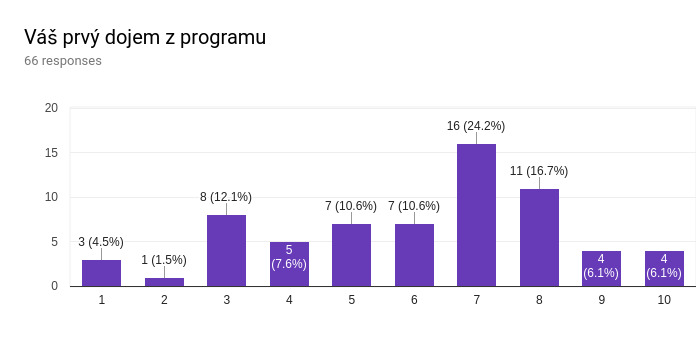
\includegraphics[width=\textwidth]{otazka12}
	\caption{Výsledky otázky č. 12}
\end{figure}

\end{document}
